\section{Simulation Results and Visualization}

This section reports a numerical run of the minimal developmental model introduced in the previous section. The aim is to show how structure appears over time in the toy system. The result is not intended as a reproduction of a specific biological process.

\subsection{Initial State}

At the initial time, the fields are nearly uniform and no organized structure is present. The morphogen field \(M\) has only a localized source term. The biological constraint-density field \(\I\) is low and has no meaningful spatial bias apart from a small perturbation. The neural commitment field \(N\) and the eye-like commitment field \(E\) are initially undifferentiated.

In this state, no information corresponding to a completed shape exists anywhere in the field.

\subsection{Time Evolution}

As the system evolves, structure appears in the following order:
\begin{enumerate}
  \item the morphogen field diffuses and forms a smooth gradient,
  \item the biological constraint-density field \(\I\) accumulates and develops spatial bias,
  \item thresholding produces a central neural-plate-like region in \(N\),
  \item the gradient magnitude \(|\nabla \I|\) defines a boundary field \(B\),
  \item the overlap of neural commitment, boundary stabilization, and a positional window produces localized eye-like commitment in \(E\).
\end{enumerate}
This process is continuous. No stage contains an encoded final drawing of the resulting structures.

\subsection{Final State}

In the final state, the simulation shows a stable central neural-plate-like region. Localized eye-like structures appear near boundary regions of the neural field. The central region itself does not produce the eye-like field, because the relevant boundary condition is weak there.

Thus, the dynamics determine both where a structure can appear and where it does not appear.

\subsection{Figure Descriptions}

Each figure corresponds to a stage in the hierarchical emergence described in the previous section.

\begin{figure}[htbp]
  \centering
  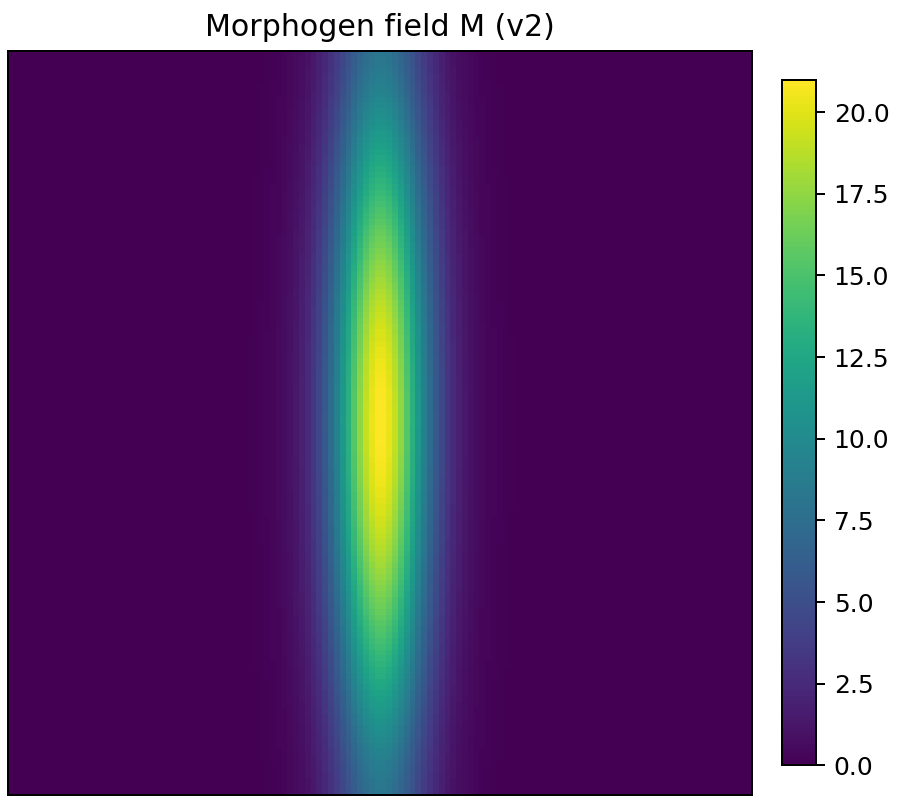
\includegraphics[width=0.70\linewidth]{simulations/minimal_neural_field/outputs/morphogen_final_v2.png}
  \caption{Final morphogen field \(M\). A smooth field forms around the central source.}
  \label{fig:sim-morphogen}
\end{figure}

\begin{figure}[htbp]
  \centering
  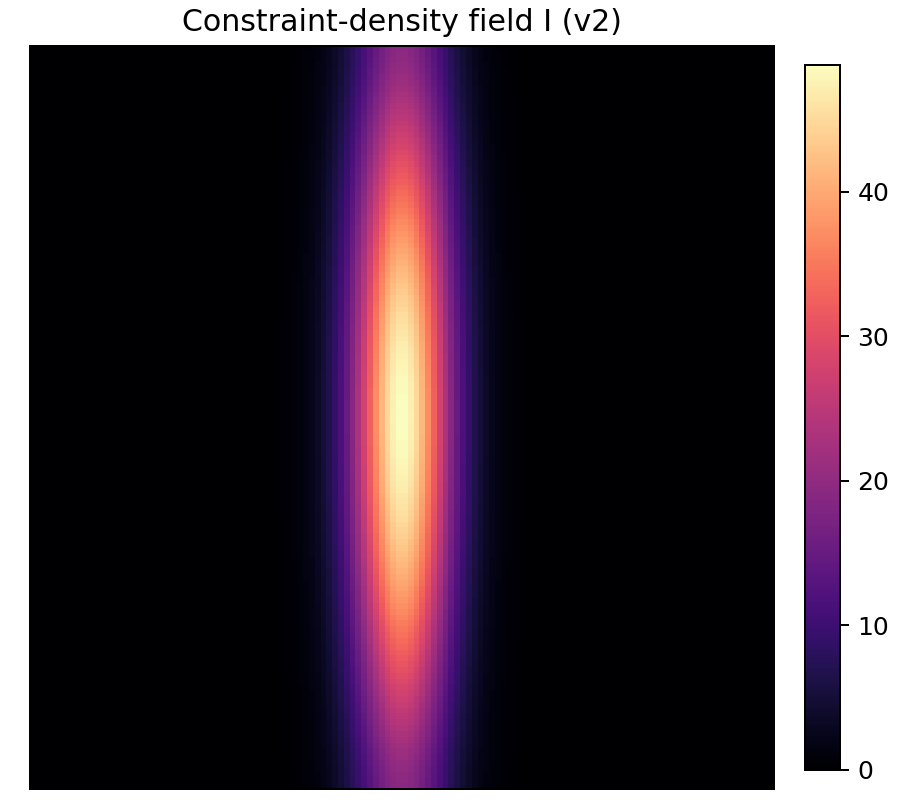
\includegraphics[width=0.70\linewidth]{simulations/minimal_neural_field/outputs/information_density_final_v2.png}
  \caption{Final biological constraint-density field \(\I\). The field accumulates in response to the morphogen field and forms a central peak.}
  \label{fig:sim-information-density}
\end{figure}

\begin{figure}[htbp]
  \centering
  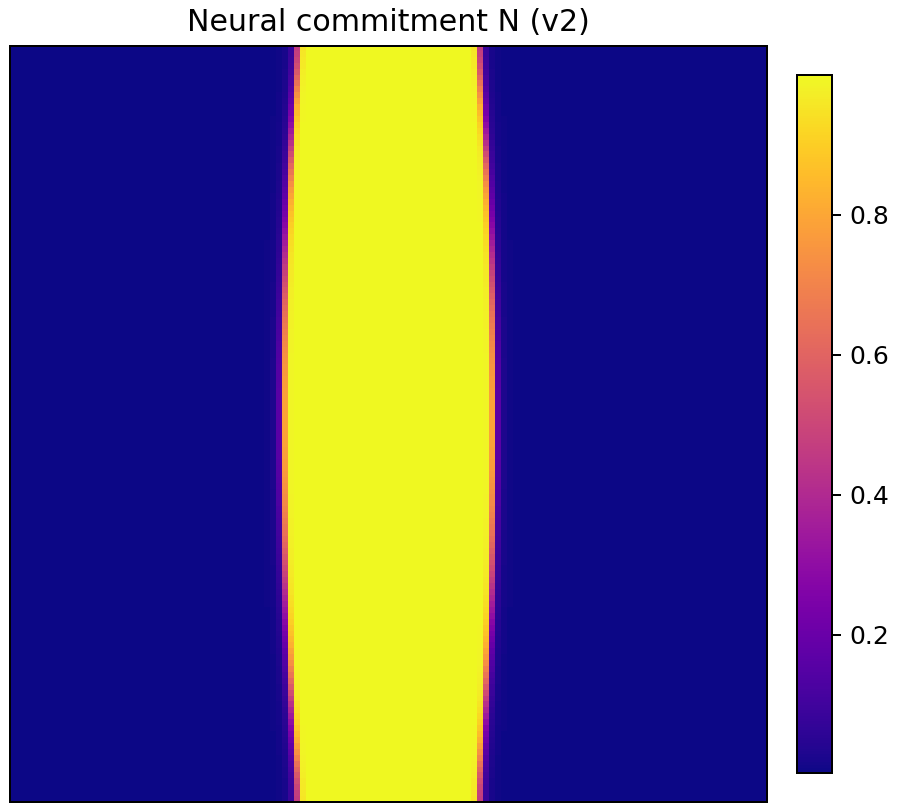
\includegraphics[width=0.70\linewidth]{simulations/minimal_neural_field/outputs/neural_commitment_final_v2.png}
  \caption{Final neural commitment field \(N\). Thresholding of biological constraint density produces a central neural-plate-like region.}
  \label{fig:sim-neural}
\end{figure}

\begin{figure}[htbp]
  \centering
  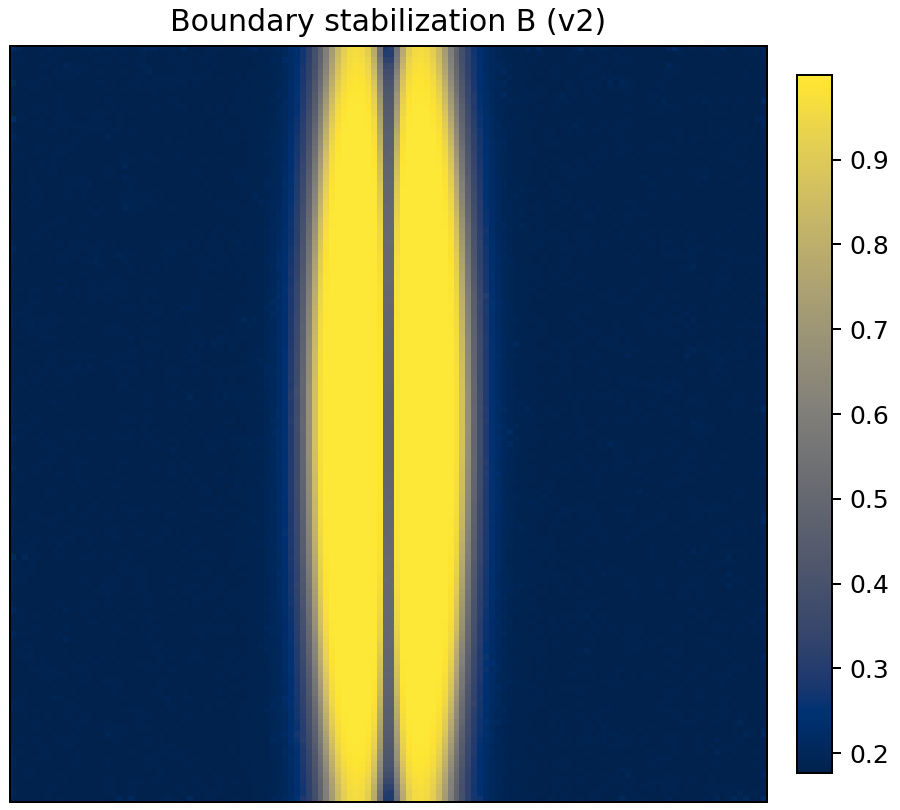
\includegraphics[width=0.70\linewidth]{simulations/minimal_neural_field/outputs/boundary_field_final_v2.png}
  \caption{Final boundary stabilization field \(B\). The field is derived from the gradient structure of \(\I\), highlighting boundary-like regions.}
  \label{fig:sim-boundary}
\end{figure}

\begin{figure}[htbp]
  \centering
  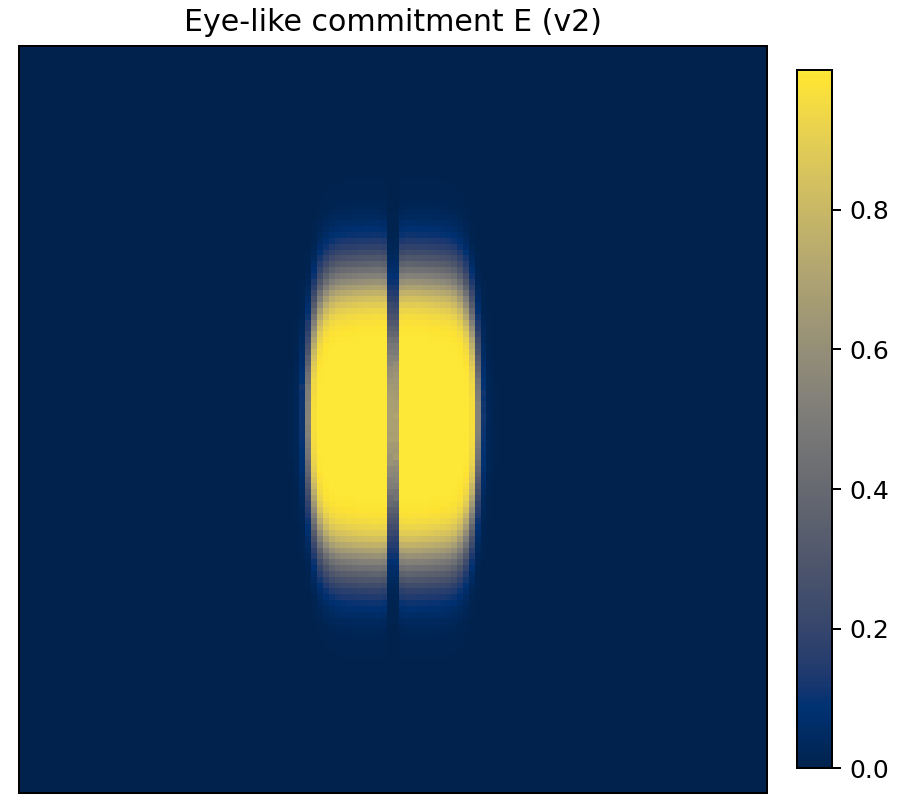
\includegraphics[width=0.70\linewidth]{simulations/minimal_neural_field/outputs/eye_commitment_final_v2.png}
  \caption{Final eye-like commitment field \(E\). Localized structures appear where neural commitment and boundary conditions overlap within the positional window.}
  \label{fig:sim-eye}
\end{figure}

\begin{figure}[htbp]
  \centering
  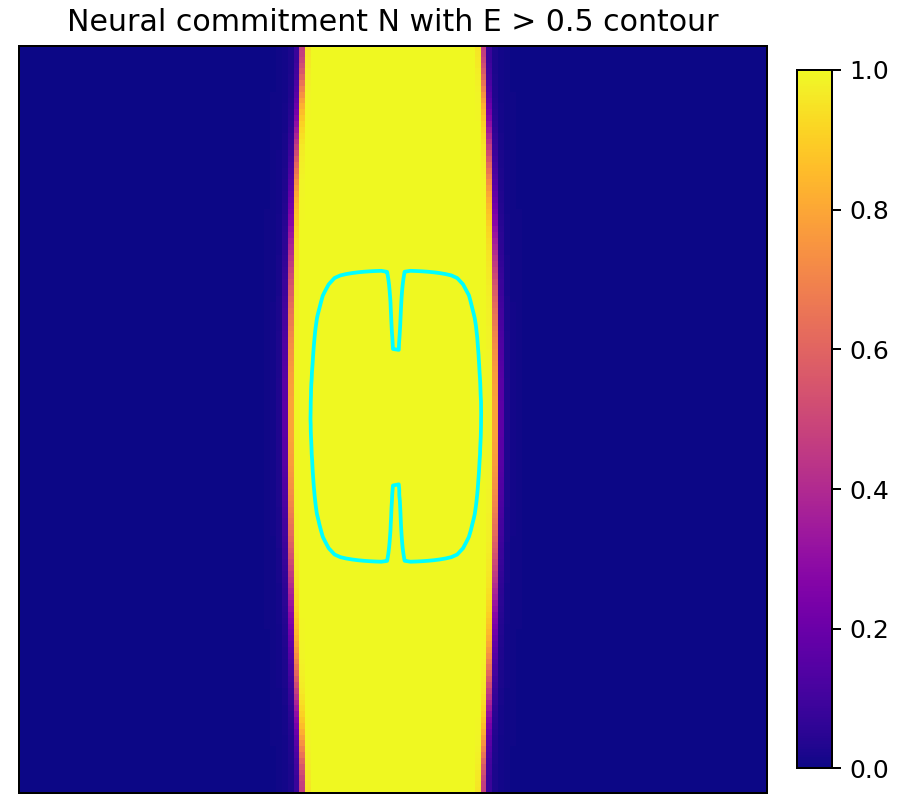
\includegraphics[width=0.70\linewidth]{simulations/minimal_neural_field/outputs/neural_eye_overlay_v2.png}
  \caption{Overlay visualization. The neural commitment field \(N\) is shown as the background, with the thresholded eye-like commitment \(E\) overlaid as a contour.}
  \label{fig:sim-overlay}
\end{figure}

\begin{figure}[htbp]
  \centering
  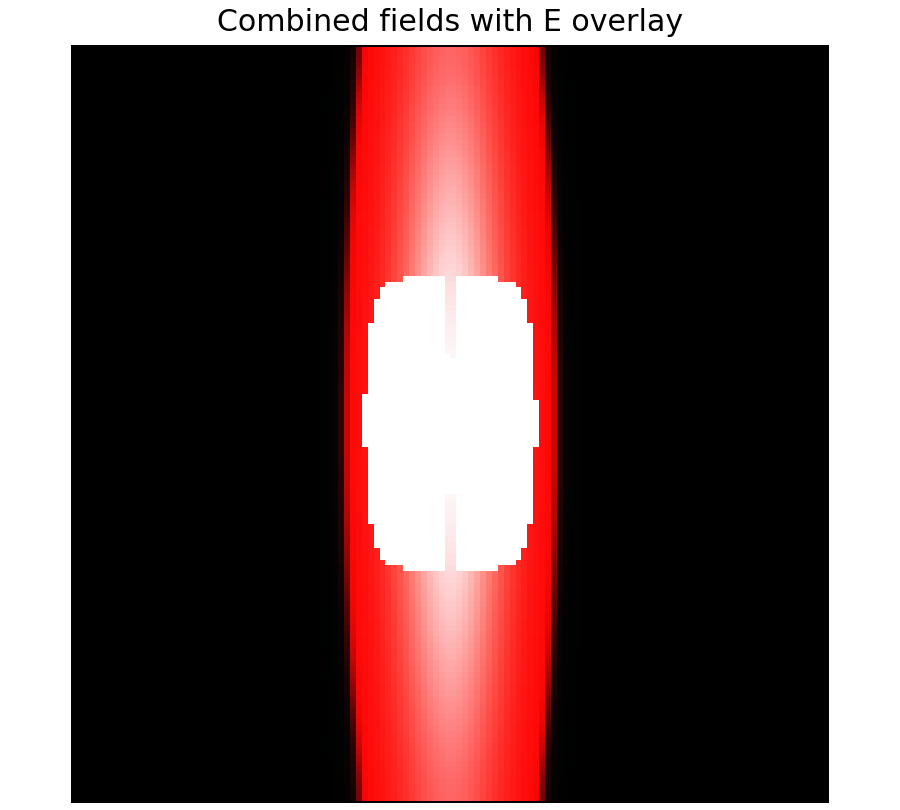
\includegraphics[width=0.70\linewidth]{simulations/minimal_neural_field/outputs/combined_fields_with_eye_v2.png}
  \caption{Combined visualization with eye-like commitment. The image summarizes the final relationship among the morphogen field, biological constraint density, neural commitment, and eye-like commitment.}
  \label{fig:sim-combined}
\end{figure}

\subsection{Time-Evolution Visualization}

The time evolution was also rendered as an animated GIF:
\begin{center}
  \path{simulations/minimal_neural_field/outputs/development_v2_hierarchical.gif}
\end{center}
Time evolution of the minimal developmental model. Structures appear as stable configurations under simple dynamical constraints.
The animation is provided as supplementary material.
The animation shows the sequence of morphogen formation, biological constraint-density accumulation, neural-plate-like stabilization, boundary extraction, and secondary eye-like commitment.

This ordering agrees with the hierarchical generation path
\begin{equation}
  M \rightarrow \I \rightarrow N \rightarrow B \rightarrow E.
\end{equation}

\subsection{Summary of Observations}

The simulation illustrates the following points:
\begin{itemize}
  \item the neural-plate-like region arises through thresholding of biological constraint density,
  \item the eye-like field arises through the combination of boundary structure and positional conditions,
  \item structure appears in stages,
  \item the final shape is not specified in advance.
\end{itemize}

The resulting structures are therefore interpreted as stable solutions under constrained dynamics.

\subsection{Role of This Section}

This result is not a model of a specific biological phenomenon. The role of the simulation is to show that structure can arise from minimal conditions in a field-based dynamical system. In this respect, the toy model is consistent with the Bio-IFGT interpretation developed in the preceding sections.

It does not demonstrate biological mechanism, but only structural possibility.

\clearpage
